\newpage
\section{Algoritmo Propuesto}\label{sec:algoritmo}
\subsection{Explicacion}

\subsubsection{Colonia de hormigas}

El algoritmo implementado esta basado en la metaheuristica de \textbf{colonia de hormigas}.

La idea general es tener una matriz que representa a la \textbf{feromona}, esta matriz reprensenta la region de entrada, en otras palabras el valor en la posicion (x,y) de la matriz de feromona representa el valor de la feromona en dicha posicion del suelo. En un principio se inicaliza con todos los valores en 0, como se ve a continuacion:


\begin{center}
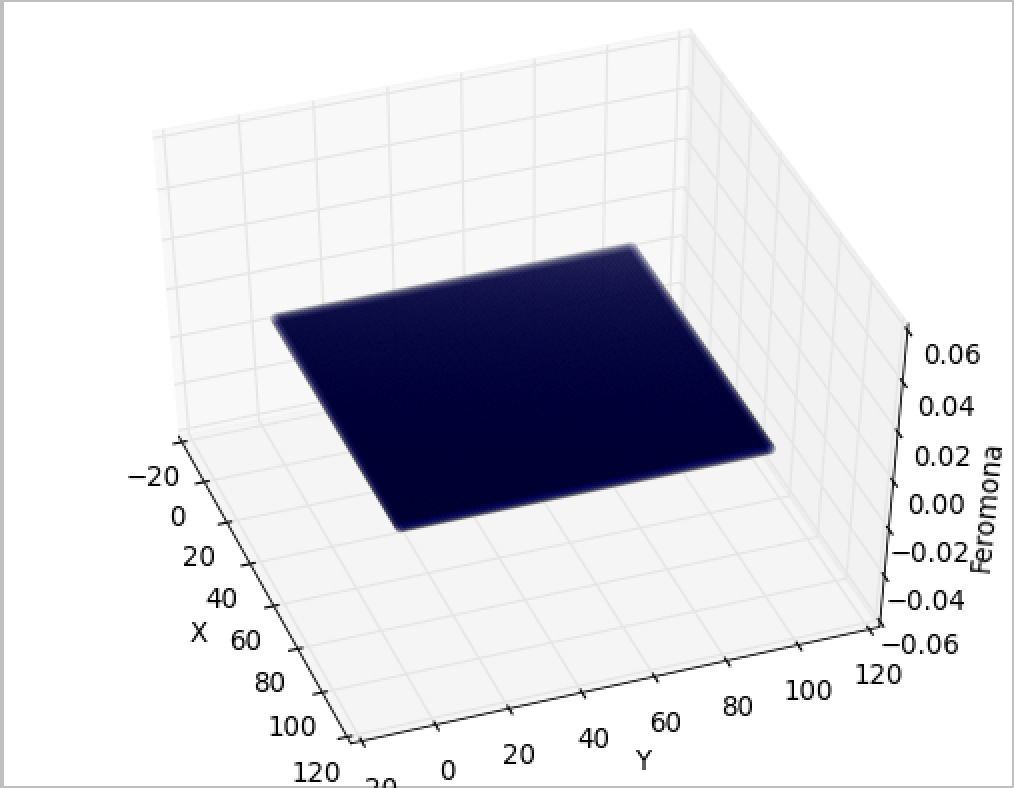
\includegraphics[width=7cm]{imagenes/feromona0}
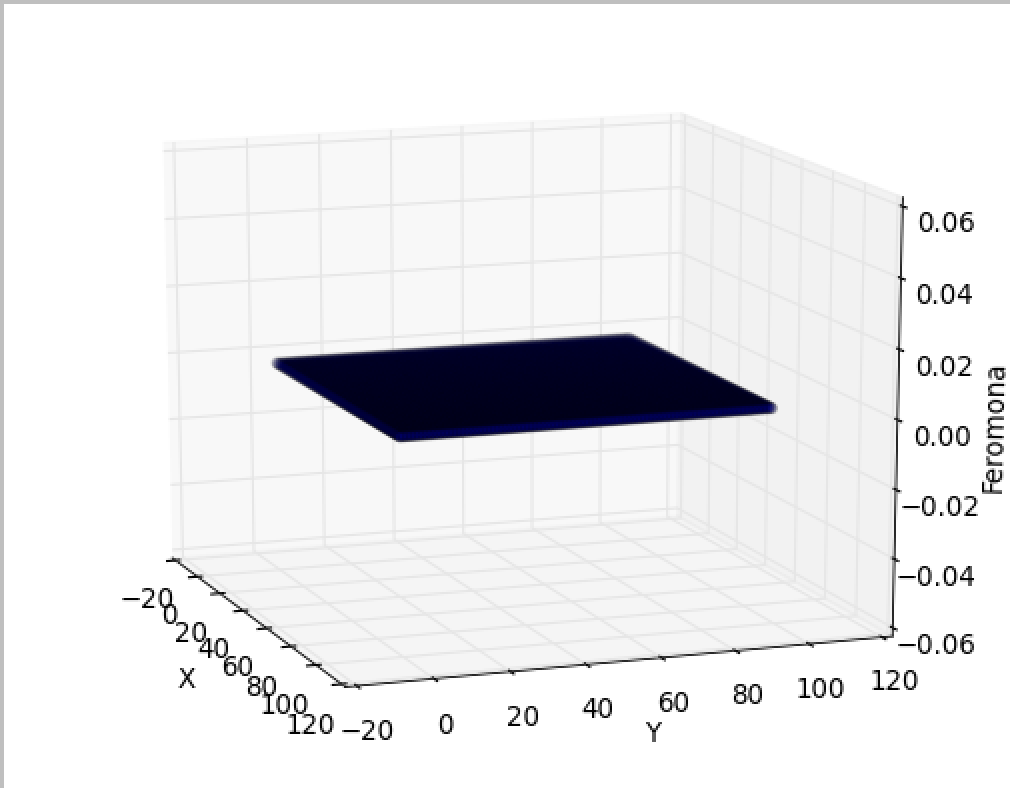
\includegraphics[width=7cm]{imagenes/feromona01}
\end{center}

La matriz de fermona esta \textbf{discretizada} con un valor \textbf{configurable por parametro}. Por ejemplo, si la region es una region de 100x100 metros, pero la discretizacion de la feromona la seteamos en 10 metros, vamos a tener una matriz de feromona de 10x10. Es clave notar en este punto que cuanto menor es el valor de la discretizacion de la feromona mayor cantidad de puntos en la matriz y por lo tanto vamos a lograr mejores resultados pero a su vez resultados con tiempo computacional mas alto (ver seccion de experiemntacion).

Por otro lado, contamos con una estructura auxiliar, una matriz de tamaños iguales que la matriz de feromona, esta estructura contiene 0 y 1 dependiendo de la \textbf{disponibilidad} del punto de la feromona. Esto es utilizado para saber cuando una feromona esta disponible, dado que los vamos a ir tapando con el correr de las iteraciones y por otro lado, en casos de que la region original no sea rectangular o este rotada, la matriz de feromona se arma de forma tal que la region quede incluida y los espacios fuera de la region se setean como \textbf{no disponibles} en esta nueva estructura. En la siguiente figura vemos un ejemplo donde la seccion amarrilla seria la region, y la azul seria la matriz de feromona, por lo tanto en la matriz de disponibilidad en los casilleros correspondientes a partes azules tendriamos un 1 indicando que no esta disponible esa feromona, ya que no esta dentro de la region.

\begin{center}
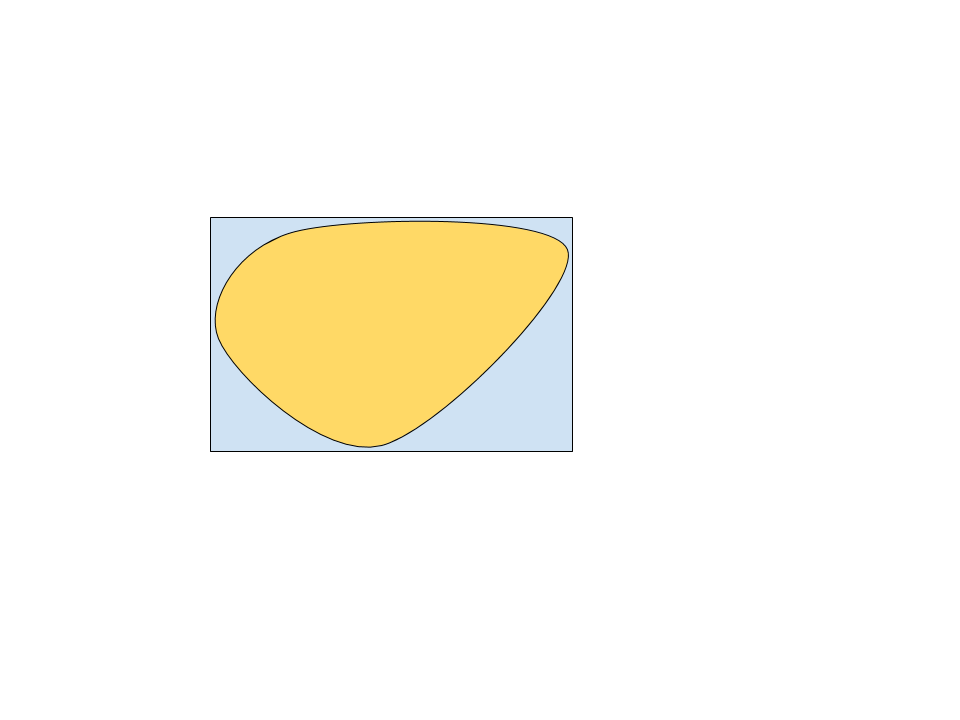
\includegraphics[width=8cm]{imagenes/ejemplo1}
\end{center}


Lo siguiente es, ejecutar una cantidad configurable de iteraciones el algoritmo obteniendo en cada solucion, un conjunto de soluciones que van \textbf{actualizando} la matriz de feromona y en cada paso del algortimo vamos \textbf{chequeando y guardandonos la mejor solucion}, siendo la mejor solucion la que tenga el valor mas alto del ogip tapado. 

En las siguientes imagenes podemos ver algunos ejemplos de feromonas luego de varias iteraciones.

\begin{center}

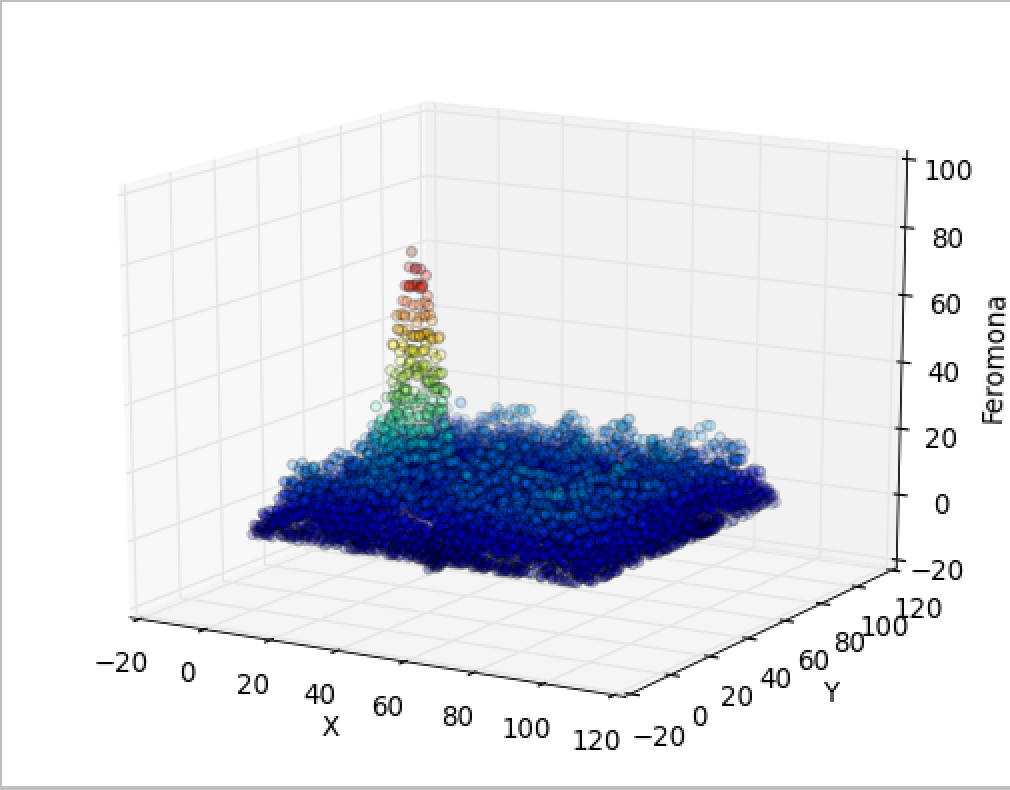
\includegraphics[width=7cm]{imagenes/fero0}
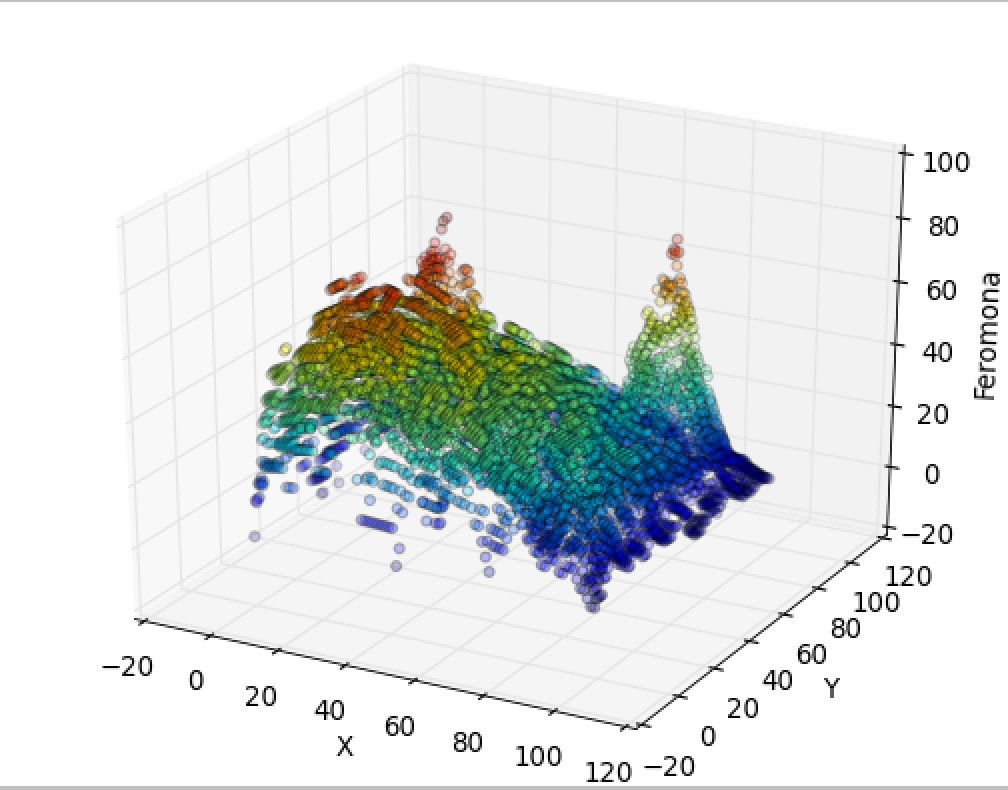
\includegraphics[width=7cm]{imagenes/fero1}
\end{center}


El algoritmo esta dividido en dos partes, la \textbf{iteracion inicial} y el \textbf{resto de las iteraciones} (decision tomado para facilitar la implementacion). 

A continuacion se explica el trabajo de cada hormiga, es decir la forma de conseguir cada solucion dependiendo si es la iteracion inicial o el resto de las iteraciones.

\textbf{Iteracion Inicial:} En esta iteracion se crean una \textbf{cantidad configurable} de soluciones random, y para cada una de estas se actualiza la matriz de feromonas de la forma que corresponda. 

Para crear una solucion random, la idea principal es meter pads centrados en puntos random de la region, teniendo en cuenta que sean validos (que esten dentro de la region, sin pisarse y sin interceptarce con una restrincion) hasta no poder meter mas pads. Notar que tambien se elije la semilla de forma random. El problema en este caso es decidir cuando ya no se pueder meter pads (dado que estamos trabajando en un plano \textbf{continuo}), por lo tanto se considero tener un \textbf{valor configurable} de intentos de meter pad fallidos. En caso de fallar en insertar el pad random esa cantidad de veces entonces se considera que no entra ningun pad mas y se retorna la solucion. 

A continuacion podemos ver un ejemplo de una solucion random, donde termino de poner pads porque se \textbf{creyo} que no entraban mas, pero podemos ver en la otra figura, marcado con amarrillo 3 posibles pads que se nota que no se encontraron.

\begin{center}
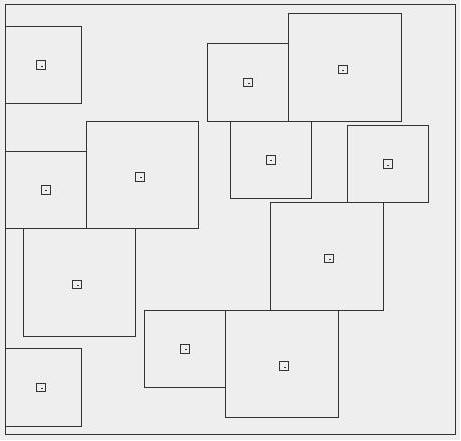
\includegraphics[width=7cm]{imagenes/ejemplo2}
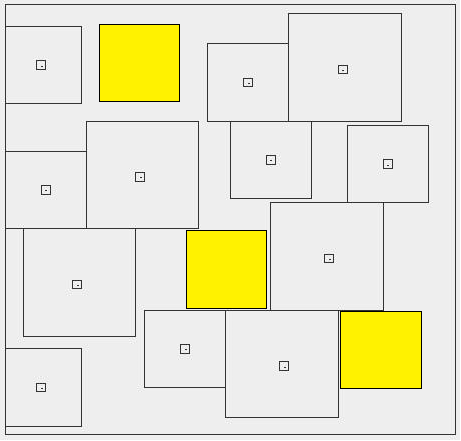
\includegraphics[width=7cm]{imagenes/ejemplo3}
\end{center}




\textbf{Resto de las iteraciones:} En esta iteracion se crean una \textbf{cantidad configurable} de soluciones no random, y para cada una de estas se actualiza la matriz de feromonas de la forma que corresponda.

Para crear una \textbf{solucion no random}, la idea principal es agarrar el punto de la feromona mas \textbf{caliente} y generar una \textbf{cantidad configurable} de pads random que puedan tapar esa feromona. 

Nota: si no consigo ningun pad random que tape dicho punto de la feromona (dado que los pads pueden ser invalidos, por ejemplo tocando una restriccion) , descarto ese punto de la feromona. 


La manera de conseguir un pad random que tape un punto c, es tan simple como un pad posicionado en cualquier lugar de la region que tape a c. \textbf{Esto esta hecho de esta forma para que cada solucion sea distinta de las otras.}

Una vez tapado el punto de la feromona, se acomoda el pad, se tapan el resto de los puntos de la feromona que este pad tapo (tambien actualizamos la matriz de disponibilidad) y se itera hasta no tener mas puntos feromona para tapar. 

\textbf{Actualizacion de la feromona:} Para actualizar la feromona utilizamos una funcion llamada \textbf{esBuenaSolucion} que determina si una solucion es buena o mala. Contamos con un \textbf{parametro configurable} dado que se tiene 3 formas distintas de ver si una solucion es buena o mala

\begin{enumerate}
\item Opcion 0: Una solucion es buena si el ogip cubierto por esta solucion es mas que el 75\% del total del ogip, en otro caso es una mala solucion.
\item Opcion 1: Una solucion es buena si el ogip cubierto por esta solucion es mas que la mitad de la suma del maximo y minimo ogip hasta el momento, en otro caso es mala solucion.
\item Opcion 2: Una solucion es buena si el ogip cubierto por esta solucon es mas que el promedio de los ogip de las soluciones calculadas hasta el momento, en otro caso es mala solucion. 
\end{enumerate}

En caso de que la solucion sea buena se recorre la matriz de feromonas, aumentanto (calentando) en cada casillero (punto de la feromona) tapado por un pad en dicha solucion un valor igual al ogip en ese punto (normalizado) por una constante configurada por parametro. Es analogo para el caso de una solucion mala, solamente que disminuyendo (enfriando).


\textbf{Importante:} Tener en cuenta que para todos los casos, una vez elegido el pad que voy a agregar a mi solucion, a este pad lo \textbf{acomodo} haciendo que se mueva para la direccion mas cercana a otro pad o borde, hasta chocarce con el. De esta forma obtengo soluciones con pad pegados entre si y no aparecen huecos.

Una vez terminadas todas las iteraciones vamos a tener guardado la mejor solucion, el numero de iteracion de donde salio dicha solucion y el tiempo en conseguirla.

Notar que la mejor solucion no necesariamente es de la ultima iteracion, es por eso que la vamos guardando en cada iteracion y tambien vamos guardando el numero y tiempo de la iteracion de donde se origino la mejor solucion.

\subsubsection{Colonia de hormigas Version Alternativa}

Tambien se desarrollo un algoritmo extra, tambien basado en \textbf{colonias de hormigas}, implementado de forma casi identica al anterior, salvo que en lugar de tener una unica matriz de feromonas, tenemos una matriz de feromonas por cada semilla, es decir si tengo 5 semillas (tipo de pad) tengo 5 matrices de fermona y una unica matriz de disponibilidad. 

Entonces a la hora de actualizar la matriz de feromona, actualizamos para cada matriz los puntos tapados por los pads que tienen esa semilla. Por ejemplo, si tenemos 2 semillas, una grande y una chica, en una matriz de feromona vamos a actualizar los puntos tapados por los pads chicos y en la otra matriz de feromona actualizamos los puntos tapados por pads grandes. 

A la hora de buscar la feromona mas caliente, se busca entre todas las matrices de feromona.

El objetivo de esto es notar la variacion de la feromona, y tratar de ver que en algunos casos es conveniente poner los pads mas grandes en los puntos mas calientes mientras que los lugares restantes, por ejemplo a los costados de los lugares de alto valor, se agregan pads mas chicos. 

A continuacion se muestran ejemplos de feromonas para esta version alternativa. Podemos ver en la figura de la izquierda como se modifico la feromona en los lugares donde tiene los pads mas grandes. Por otro lado, la feromona de la derecha se nota como esta modificada en los lugares que rodean a los pads mas grandes, concluyendo que se pusieron pads mas chicos en los alrededores de los mas grandes (ver seccion experiementacion)

\begin{center}

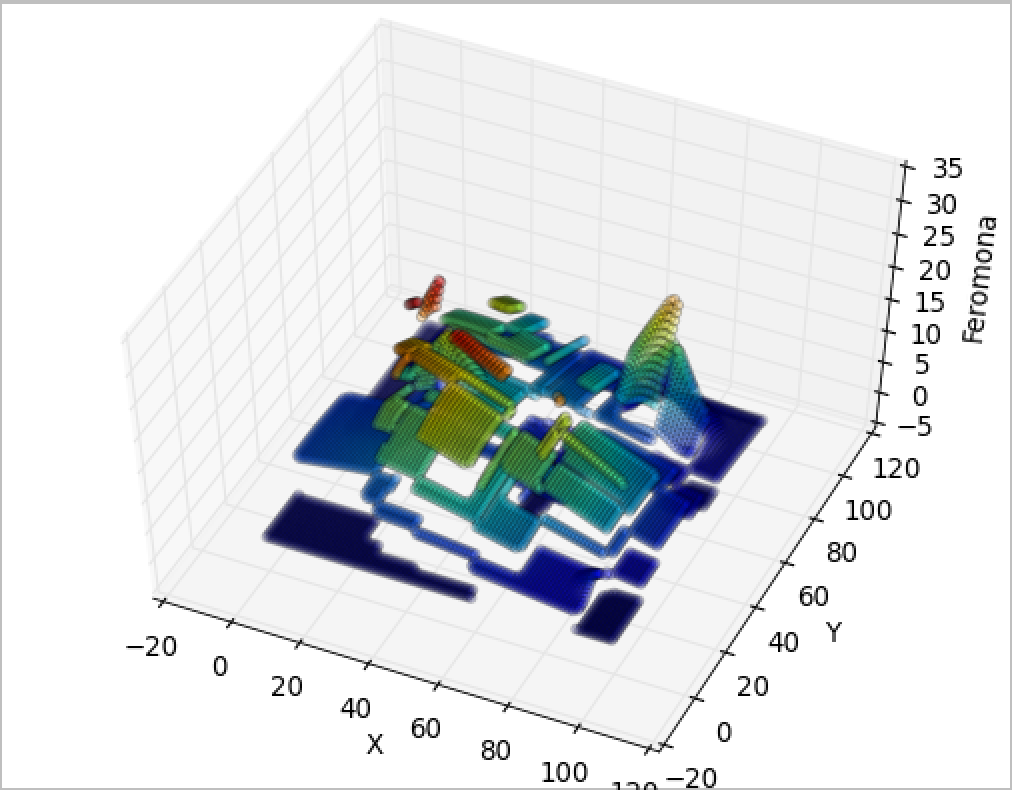
\includegraphics[width=7cm]{imagenes/ferov20}
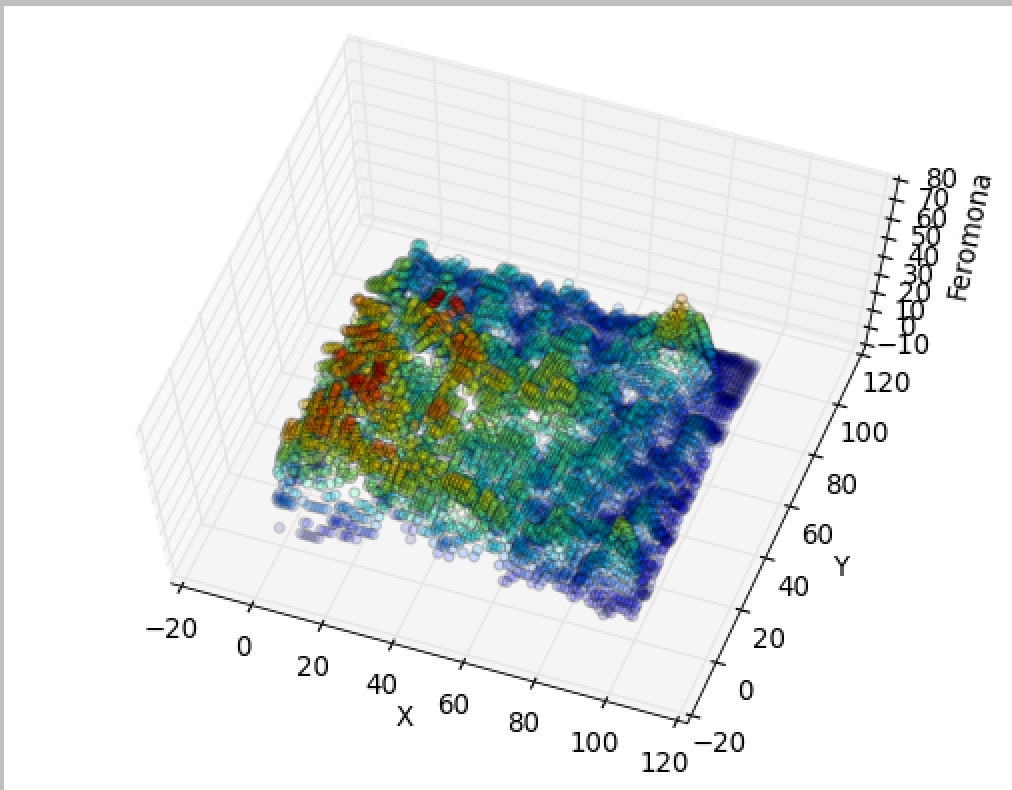
\includegraphics[width=7cm]{imagenes/ferov21}
\end{center}

A continuacion podemos ver algunos ejemplos de soluciones obtenidas sobre una misma instancia cambiando los parametros (ver mas en seccion experimentacion).

\begin{center}

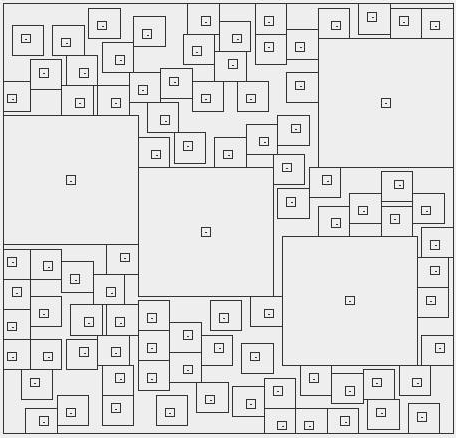
\includegraphics[width=7cm]{imagenes/ejemplo7}
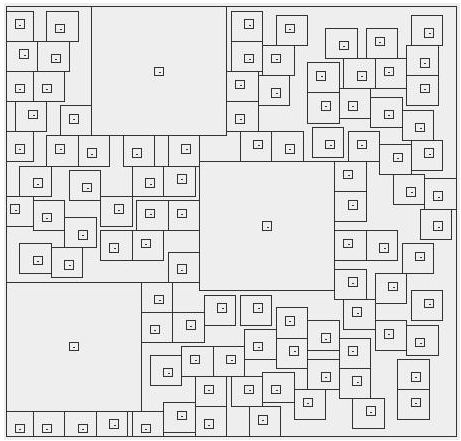
\includegraphics[width=7cm]{imagenes/ejemplo5}
\end{center}


\begin{center}
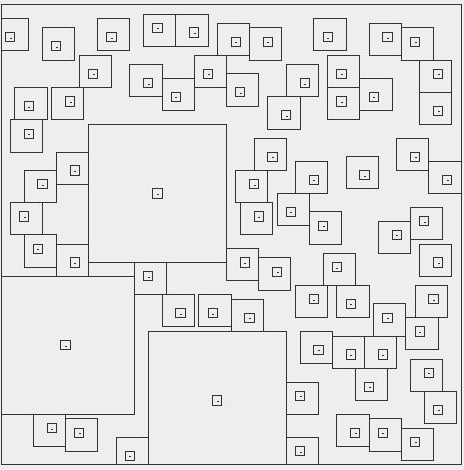
\includegraphics[width=7cm]{imagenes/ejemplo6}
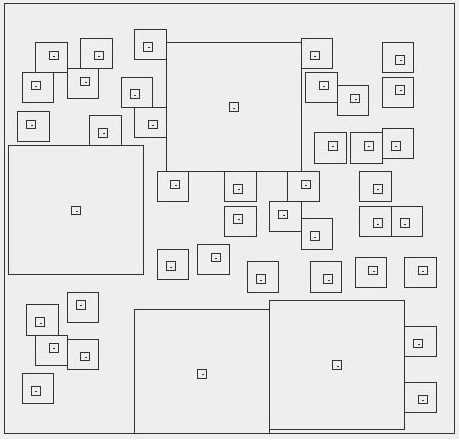
\includegraphics[width=7cm]{imagenes/ejemplo4}

\end{center}

Notar que en los dos primeros casos no quedaron huecos mientras que en los ultimos dos si, esto se debe a la discretizacion de la feromona (en los ultimos dos casos la discretizacion es un numero mas alto, por lo tanto tenemos menos lugares que tapar, provocando huecos).

\newpage


\subsection{Pseudocodigo}
\subsubsection{Algoritmo principal}

\begin{verbatim}
    resolver() {
        inicializarFeromonas();
        ejecutarIteracionInicial();
        return ejecutarProximasSoluciones();
    }
\end{verbatim}

\textbf{InicializarFeromonas()} es una funcion que inicializa la feromona como una matriz del tamanio de la region, en caso que la region no se rectangular la inicializa con el rectangulo mas chico que contenga a la region. 

Tambien inicializa una matriz disponibilidad del mismo tamanio que la feromona pero esta contiene 1 o 0 diciendonos si una feromona es validad o no, sea porque ya esta usada o porque la region es mas chica que la matriz de feromonas y en esa feromona no tenemos region.


\begin{verbatim}
    ejecutarIteracionInicial() {
        soluciones = crearSolucionesRandom();
        for (Solucion solucion : soluciones) {
            if(esBuenaSolucion()){
                actualizarFeromona(solucion, OperacionFeromona.Calentar);
            } else {
                actualizarFeromona(solucion, OperacionFeromona.Enfriar);
            }
        }
    }
\end{verbatim}		

\textbf{ejecutarIteracionInicial()} crea una cantidad seteada por parametro de soluciones randoms y para solucion chequea si es una buena o mala solucion, la funcion \textbf{esBuenaSolucion()} cambia segun un valor pasado por parametro, pero en definitiva, devuelve \textbf{true} si es una solucion considerada buena o \textbf{false} si es considerada mala. 

En caso de que la solucion sea buena, \textbf{calentamos} la matriz de feromonas y \textbf{enfriamos} en caso contrario.

La funcion \textbf{actualizarFeromona()} simplemente recorre la matriz \textbf{calentando} o \textbf{enfriendo} cada valor respectivamente. Pero notar que la calienta \textbf{teniendo en cuenta el valor del ogip en ese punto}, es decir, se normaliza el ogip y en cada punto de feromona se calienta o enfria un valor igual a $escalar * feromonaNormalizadaEnElPunto$. Esto es para que el algoritmo de colonias de hormigas tenga en cuenta los valores originales del problema para generar sus soluciones.


La funcion \textbf{esBuenaSolucion()}, tiene 3 opciones que se cambian dependiendo de un valor pasado por parametro

\begin{enumerate}
\item Opcion 0: Una solucion es buena si el ogip cubierto por esta solucion es mas que el 75\% del total del ogip, en otro caso es una mala solucion.
\item Opcion 1: Una solucion es buena si el ogip cubierto por esta solucion es mas que la mitad de la suma del maximo y minimo ogip hasta el momento, en otro caso es mala solucion.
\item Opcion 2: Una solucion es buena si el ogip cubierto por esta solucon es mas que el promedio de los ogip de las soluciones calculadas hasta el momento, en otro caso es mala solucion. 
\end{enumerate}



\begin{verbatim}	
crearSolucionesRandom() {
    ret = new Solucion()
    while (hasta que el area deje de cambiar) {
        Coordenada c = generarCoordenadaRandom()
        Pad pad = crearPadConSemillaRandamCentradaEnCoordenada(c)
        if (padValido(pad)){
            Pad padAcomodado = acomodarPad(pad);
            agregarPadASolucion(ret,padAcomodado);
        }
    }
    return ret;
}
\end{verbatim}	

La condicion del while corta cuando ya no se pueden meter mas pads en mi solucion random, esto se hace teniendo en cuenta una cantidad fijada por parametro de intentos de meter un pad, es decir, intento meter pads en la solucion y si la cantidad de veces que no pude meter es mayor al parametro seteado, se asume que no entran mas pads y sale del while. 

Esto se hace para tratar de manejar la region en un plano \textbf{continuo} y para tratar de solucionar el problema de saber cuando ya no entran mas pads.

\textbf{GenerarCoordenadaRandom()} generada un x,y random dentro de la region. 

\textbf{crearPadConSemillaRandamCentradaEnCoordenada(c)()} elije una semilla random y crea un pad centrado en c

\textbf{padValido(pad)} chequea si el pad no se pisa con ninguna restrincion, ni se va fuera de la region, ni se pisa con otro pad ya agregado a la solucion.

\textbf{acomodarPad(pad)} mueve el pad para una direccion random hasta chocarce son un borde u otro pad sin destapar el centro. Eso se hace para tratar de pegar todos los pads en la solucion.

\textbf{agregarPadASolucion()} agrega el pad a la solucion.

\textbf{ejecutarProximasSoluciones()} ejecuta una cantidad de veces igual a \textbf{cantIteraciones}, un algoritmo similar a \textbf{crearSolucionesRandom()}, llamado \textbf{generarSolucionesMaximaTemperatura()}. De esta forma se crean soluciones durante muchas iteraciones.

\textbf{generarSolucionesMaximaTemperatura()} es exactamente igual a \textbf{crearSolucionesRandom()} nada mas que cambiando el metodo \textbf{crearSolucionesRandom()} por \textbf{generarSolucionesMaximaFeromona()}. Esto significa que crea una cantidad configurable de soluciones de maxima feromona. Y para cada solucion chequea si es buena o mala actualizando la feromona como corresponda al igual que lo haciamos en la iteracion inicial.

Una solucion de maxima feromona es una solucion que tiene en cuenta el valor de la fermona para generarse y se genera con el siguiente algoritmo:


\begin{verbatim}
construirSolucionMaximaTemperatura() {
    sol = new Solucion();
    while (mientra que tenga feromonas disponibles) {
        Feromona p = getMaximaFeromona()
        if (es una feromona que se puede tapar) {
            for (int j = 0; j < getCantIntentosTaparFeromona(); j++) {
                nuevoPad = generarNuevoPad(p);
                if (esPadValido(nuevoPad)) {
                    nuevoPad = acomodarPad(nuevoPad);
                    agregarPadASolucion(nuevoPad);
                    break;
                }
            }
        }
    }
    return sol;
}
\end{verbatim}

Mientras tenga feromonas disponible, es decir que todavia no las tapas (y estan dentro de la region) ejecuto todo el codigo dentro del while. 

Obtengo la maxima feromona con \textbf{getMaximaFeromona()} y chequeo si es una posible feromona a tapar, dado que podria pasar que esa feromona este en una restrincion. 
Una vez que ya se que esa feromona la puedo tapar, trato de generar \textbf{getCantIntentosTaparFeromona()} pads (este valor es seteado por parametro). 

La idea general es que para cada iteracion genero un pad random que tape a la feromona, chequeo si es valido, y si es valido lo agrego a la solucion y dejo de intentar tapar esta feromona.

Si no encontre ningun pad que sea valido y tape a la feromona en \textbf{getCantIntentosTaparFeromona()} intentos entonces ya esa feromona la descarto. 

\textbf{Notar que a los pads los acomodo (al igual que antes) para que queden pegados a otros pads o al borde.}

\textbf{Nota importante:} Tanto en la generacion de soluciones random o las soluciones de maxima feromona, a la hora de fijarse si es una buena o mala solucion para actualizar la feromona, se chequea si es la \textbf{mejor solucion}, en caso de ser la mejor se \textbf{guarda}. Esto es para guardar la mejor solucion en el camino, podria llegar a pasar que la mejor solucion la encuentre en iteraciones iniciales y las siguientes sean peores.


\subsubsection{Alternativa: Muchas Feromonas}
A parte de tener un algoritmo de colonias de hormigas que ejecuta con una unica feromona, se programo una version alternativa donde contamos con mas de una feromona. Es decir para cada solucion, en lugar de tener una unica feromona, \textbf{tenemos una matriz de feromona para cada semilla}.
 
Para esto se modifica leventente el codigo teniendo en cuenta que ahora manejamos arrays de feromonas, y cambian levemente los algoritmos de actualizar la feromona. En particular, el algoritmo para obtener cual es la maxima feromona es el siguiente:


\begin{verbatim}
getMaximaFeromona() {
    result = null;
    for (f in todas las feromonas) {
        if(si la feromona f tiene valores dissponibles)
            if(maximo de f > result)
                result = f1;
    }
    return result;
}
\end{verbatim}

El algoritmo es bastante sencillo, la idea es recorrer todas las feromonas buscando el maximo valor. 

Tener en cuenta que a la hora de actualizar la feromona, cada feromona solo se actualiza donde corresponde. Por ejemplo,  la feromona correspondiente a la semilla 0 se calienta o enfria solo en los puntos donde la solucion puso semillas 0. 